\documentclass[11pt,a4paper]{article}
\usepackage[margin=2.6cm]{geometry}
\usepackage{amsmath,amssymb}
\usepackage{booktabs,array}
\usepackage{enumitem}
\usepackage{xcolor}
\usepackage{tikz}
\usepackage{pgfplots}
\pgfplotsset{compat=1.17}
\usepackage[colorlinks=true,linkcolor=teal!70!black,citecolor=teal!70!black,urlcolor=teal!70!black]{hyperref}

\definecolor{bandA}{HTML}{008A7C}
\definecolor{bandB}{HTML}{C2610C}
\newcommand{\tagbox}[2]{\textsf{\scriptsize\colorbox{#1!12}{\textcolor{#1!70!black}{#2}}}}
\newcommand{\est}{\tagbox{gray}{established}}
\newcommand{\lit}{\tagbox{blue}{literature}}
\newcommand{\ours}{\tagbox{orange}{ours}}
\newcommand{\lP}{\ell_{\mathrm P}}

\title{Is It Spacetime?\\[4pt]
\large Discrete universes measured by counting: a cosmological cutoff, a manifold detector,\\ and a first look at quantum weights}
\author{Draft v3 --- internal notebook checkpoint}
\date{25 October 2026\\[2pt]\small Not for circulation. Claims are tagged \est, \lit{} or \ours.}

\begin{document}
\maketitle

\begin{abstract}
We model spacetime as a discrete set of events with a causal order and nothing else, and ask two questions: how much geometry can be read off the order by counting alone, and which ways of producing such universes give something that looks like spacetime. First, Lorentz-invariant discreteness gives every event one neighbour per unit of rapidity, a known result. We take the finite size of the universe as the physical cutoff, which caps the rapidity at $\eta_{\max}\approx142$ and singles out the cosmological frame. Second, we assemble a toolkit for $1+1$ dimensions that uses only counts. Proper time comes from the longest chain. Spatial distance comes from the causal overlaps of Boguñá and Krioukov, for which we find an exact $1+1$ identity, $d^2=2V_AV_B/V_C$, valid for any reference event in the common past; it recovers distances to $2.5$--$5\%$. In curved spacetime the same estimate drifts with the depth of the reference event as $1-R\tau^2/16$, which we use to measure curvature. A Lorentzian multidimensional-scaling embedding then recovers flat positions to better than one event spacing and acts as a ``manifold detector'' through its eigenvalue spectrum, once a universe has at least $100$--$200$ events. Third, we apply the detector. Universes grown event by event fail it. Universes weighted by $e^{-\beta S}$, with $S$ the Benincasa--Dowker action, pass it in the continuum phase and fail it in the layered crystal phase. With quantum weights $e^{i\beta S}$, estimated by sampling at $N=100$, interference does not follow the classical drift away from manifold-like universes for $\beta\le0.3$. This agrees with exact sums at $N\le9$, but the effect is at the level of fluctuations and needs larger runs. Gravity in $3+1$ dimensions and matter are still absent.
\end{abstract}

\section{The question and the rules}
In 1900 Planck assumed that energy comes in discrete quanta. We ask the analogous question for spacetime: can it be a discrete set of events that only \emph{looks} continuous from far away, with general relativity (GR) as its large-scale description? The working constraints are:
\begin{enumerate}[label=\textbf{C\arabic*},leftmargin=*,itemsep=1pt]
\item \textbf{Discrete spacetime.} Events and the causal order between them; the continuum is a large-scale limit.
\item \textbf{No background.} No absolute space and no fixed aether; every statement is about relations between events.
\item \textbf{Non-locality regulated by the finite size of the universe} (Sec.~\ref{sec:cutoff}).
\item \textbf{Local Lorentz invariance} for all boosts well below the cutoff.
\item \textbf{A cosmological clock computed from the universe's own state}, e.g.\ the longest chain back to the beginning. It may be used as a bookkeeping clock for growth, but local laws must not depend on it, and predictions must not depend on which relational clock is used. Its frame should coincide with the matter (CMB) frame \est; that is a test, not an input.
\item \textbf{Newton and Einstein from far away.}
\item \textbf{Creation (and perhaps destruction) of events drives expansion}, possibly through quantum creation operators.
\item \textbf{The links between events are quantum.}
\end{enumerate}
Missing so far is \emph{matter}: nothing in the model yet plays the role of what gravitates.

A \emph{fixed background} is structure the laws refer to but which nothing affects; C2 forbids it. A \emph{dynamical preferred-frame field}, such as the Einstein-aether~\cite{JacobsonMattingly01}, breaks local Lorentz invariance. A \emph{preferred frame of the state}, such as the CMB frame, comes from the contents of the universe while the laws stay invariant. C5 allows only the last kind.

\paragraph{The storyline.} Section~\ref{sec:cutoff} explains why the finite size of the universe is our regulator. A discrete universe is only useful if it looks like spacetime, so Sec.~\ref{sec:toolkit} builds tools that answer ``is it spacetime?'' from the order alone, and Sec.~\ref{sec:which} applies them to three ways of producing universes: classical growth, $e^{-\beta S}$ weights and quantum weights.

\section{Neighbours and the cosmological cutoff}\label{sec:cutoff}
\paragraph{One neighbour per unit of rapidity.} \lit{} Following causal set theory~\cite{BLMS87,Surya19}, $y$ is a \emph{neighbour} (a \emph{link}) of $x$ if $y$ is in the causal future of $x$ and no other event lies causally between them. In $1+1$ dimensions, with density $\rho$, write a future event as $u=t-x=\tau e^{-\eta}$, $v=t+x=\tau e^{\eta}$, where $\tau$ is the proper time from the origin and $\eta$ the rapidity. The area element is $dt\,dx=\tau\,d\tau\,d\eta$, and the interval up to the event has area $\tau^2/2$, so it is empty with probability $e^{-\rho\tau^2/2}$. Therefore
\begin{equation}
\langle N_{\rm links}\rangle=\int d\eta\int_0^\infty \rho\,\tau\,e^{-\rho\tau^2/2}\,d\tau=\int d\eta\cdot 1 .
\label{eq:onepereta}
\end{equation}
There is one expected neighbour per unit of rapidity, so an infinite universe gives every event infinitely many neighbours. This is the elementary core of the Bombelli--Henson--Sorkin theorem~\cite{BHS06}: Lorentz-invariant discreteness is non-local~\cite{Sorkin07}.

\paragraph{A finite universe caps the rapidity.} \ours{} A neighbour at proper time $\tau$ and rapidity $\eta$ lies at distance $r\approx(\tau/2)e^{\eta}$. In a universe of size $L$ this cannot exceed $L$, so
\begin{equation}
\eta_{\max}\simeq\ln\frac{2L}{\lP}\approx142,
\end{equation}
with $L\approx4.4\times10^{26}$\,m and $\lP=1.6\times10^{-35}$\,m. Lorentz kinematics has been tested up to $\eta\approx25$--$27$ (GZK protons and the highest-energy cosmic rays~\cite{CG99}), far below the cutoff. The only frame singled out is that of the universe as a whole, a frame of the state, as C5 requires. In $1+1$ dimensions an event has about $2\eta_{\max}\approx280$ future neighbours. In $3+1$ dimensions the cutoff leaves $\sim(L/\lP)^2\approx10^{124}$ (Appendix~\ref{app:dropped} lists the numerology we avoid).

\section{Geometry by counting}\label{sec:toolkit}
Everything in this section uses only the causal order. To test the tools we generate universes by Poisson sprinkling at density $\rho$ into a known spacetime, discard the coordinates, and compare what the tools find with the truth. We write $\ell=\rho^{-1/2}$ for the discreteness length in $1+1$ dimensions: a patch of volume $\ell^2$ holds one event on average.

\subsection{Time: the longest chain}
\lit{} The proper time between two events is estimated by the longest chain between them~\cite{BrightwellGregory91}. In a sprinkled $1+1$ diamond this is the longest increasing subsequence of a random permutation, with mean $\simeq2\sqrt n$ and Tracy--Widom fluctuations $\simeq0.90\,n^{1/6}$~\cite{BDJ99}, so $\delta\tau/\tau\simeq0.45\,n^{-1/3}$. Our simulations reproduce both (\texttt{sims/causal\_diamond.py}). Equivalently $\tau^2=2V$, where the volume $V$ of the interval is its number of events divided by $\rho$. \ours{} (interpretation) Geometry measured by counting is intrinsically fuzzy. The fuzziness is a relation between events, not a smearing in a background space.

\subsection{Space: causal overlaps and a rectangle identity}
\lit{} For two events $a,b$ with neither before the other, Boguñá and Krioukov~\cite{BK24} pick an event $c$ in their common past and compare the intervals $I(c,a)$ and $I(c,b)$:
\begin{equation}
A=I(c,a)\setminus I(c,b),\quad B=I(c,b)\setminus I(c,a),\quad C=I(c,a)\cap I(c,b),\qquad O=\frac{V_C}{\min(V_A,V_B)+V_C}.
\end{equation}
With $c$ chosen at equal proper time $\tau_c$ from $a$ and $b$, in $1+1$ dimensions $d=\tau_c(1-O)/\sqrt O$. We re-derived this.

\begin{figure}[t]
\centering
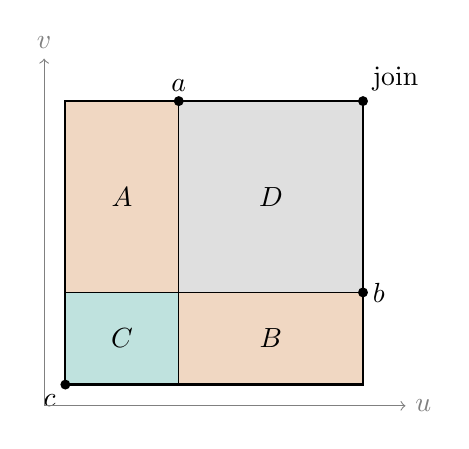
\begin{tikzpicture}[scale=0.9]
  \fill[bandA!25] (0,0) rectangle (1.6,1.3);
  \fill[bandB!25] (0,1.3) rectangle (1.6,4);
  \fill[bandB!25] (1.6,0) rectangle (4.2,1.3);
  \fill[gray!25] (1.6,1.3) rectangle (4.2,4);
  \draw[thick] (0,0) rectangle (4.2,4);
  \draw (1.6,0) -- (1.6,4); \draw (0,1.3) -- (4.2,1.3);
  \node at (0.8,0.65) {$C$}; \node at (0.8,2.65) {$A$}; \node at (2.9,0.65) {$B$}; \node at (2.9,2.65) {$D$};
  \fill (0,0) circle (2pt) node[below left] {$c$};
  \fill (1.6,4) circle (2pt) node[above] {$a$};
  \fill (4.2,1.3) circle (2pt) node[right] {$b$};
  \fill (4.2,4) circle (2pt) node[above right] {join};
  \draw[->,gray] (-0.3,-0.3) -- (4.8,-0.3) node[right] {$u$};
  \draw[->,gray] (-0.3,-0.3) -- (-0.3,4.6) node[above] {$v$};
\end{tikzpicture}
\caption{The rectangle identity in light-cone coordinates (rotate by $45^\circ$ for the usual picture). The rectangle from $c$ to the join of $a$ and $b$ splits into four tiles: the overlap $C$, the strips $A$ and $B$ seen by only one of $a,b$, and the diamond $D$ with $a$ and $b$ at its corners. Opposite tiles have equal products, $C\cdot D=A\cdot B$, and $D$ encodes the distance between $a$ and $b$.}
\label{fig:tiles}
\end{figure}

\ours{} In $1+1$ dimensions the choice of $c$ does not matter. Step by step (Fig.~\ref{fig:tiles}):
\begin{enumerate}[leftmargin=*,itemsep=1pt]
\item In light-cone coordinates $dt\,dx=du\,dv/2$, and for spacelike events $d^2=\Delta x^2-\Delta t^2=-\Delta u\,\Delta v$.
\item With $c$ at the origin, $I(c,a)=[0,u_a]\times[0,v_a]$ and $I(c,b)=[0,u_b]\times[0,v_b]$ are rectangles. Take $u_a<u_b$, $v_a>v_b$.
\item The rectangle from $c$ to the join $(u_b,v_a)$ splits into $C=[0,u_a]\times[0,v_b]$, $A=[0,u_a]\times[v_b,v_a]$, $B=[u_a,u_b]\times[0,v_b]$ and $D=[u_a,u_b]\times[v_b,v_a]$.
\item Opposite tiles have equal products: $C\cdot D=u_av_b\,\Delta u\,\Delta v=A\cdot B$.
\item $D$ has $(u,v)$-area $|\Delta u\,\Delta v|=d^2$, hence volume $d^2/2$.
\end{enumerate}
Therefore, for \emph{any} $c$ in the common past,
\begin{equation}
d^2=\frac{2\,V_AV_B}{V_C}\;\approx\;\frac{2\,N_AN_B}{\rho\,(N_C+1)} .
\label{eq:rect}
\end{equation}
The strips $A$ and $B$ are long and thin, so they hold many events even when $d\sim\ell$; this is also why the Boguñá--Krioukov estimator works at short distances. Their equal-time choice is the special case $V_A=V_B$. The identity holds only in $1+1$ dimensions, because in more dimensions the overlap of two diamonds is not a diamond. The counts $N_A,N_B,N_C$ come from disjoint regions and are therefore independent Poisson variables. $N_AN_B$ is then unbiased, but $1/N_C$ is not; $1/(N_C+1)$ has mean $(1-e^{-\lambda})/\lambda$ and removes the bias. Before this fix, a flat control read $+11\%$.

\begin{table}[t]
\centering\small
\begin{tabular}{@{}rccc@{}}
\toprule
$N$ & $d<2\ell$ & $2\ell$--$10\ell$ & $>10\ell$\\
\midrule
1000 & 23\% & 6.5\% & 5.2\%\\
2000 & 15\% & 5.0\% & 3.4\%\\
4000 & 19\% & 5.1\% & 2.5\%\\
\bottomrule
\end{tabular}
\caption{Median relative error of Eq.~\eqref{eq:rect} with the deepest $c$, flat $1+1$ sprinklings, 4 seeds (\texttt{sims/s4a\_overlap\_distance.py}). There is no significant bias above $2\ell$. The large-distance error falls roughly as $N^{-1/2}$. Below $2\ell$ the error stays at $\sim20\%$: this is the discreteness scale.}
\label{tab:dist}
\end{table}

\subsection{Curvature: the estimate drifts with depth}
\lit{} Curvature can be read from counts through the Benincasa--Dowker operator~\cite{BD10,DowkerGlaser13}. In our runs (session 2) it gave the right sign and order of magnitude for de Sitter, but was noisy at $10^4$ events. Related continuum results give the curvature corrections to the volume of a small causal diamond~\cite{GibbonsSolodukhin07} and to chain counts inside it~\cite{RSS13}.

\ours{} The rectangle identity provides a second route. Two-dimensional de Sitter space, $ds^2=(H\eta)^{-2}(-d\eta^2+dx^2)$, has the same light cones as flat space, so $A,B,C,D$ are the same rectangles, but volumes are weighted by $dV=2\,du\,dv/(H^2(u+v)^2)$. Integrating over a rectangle gives a logarithm of the conformal times at its corners,
\begin{equation}
V_\square=\frac{2}{H^2}\ln\frac{\eta_L\,\eta_R}{\eta_{\rm bottom}\,\eta_{\rm top}},
\end{equation}
and $C\cdot D=A\cdot B$ no longer holds exactly. For $a,b$ on one slice and $c$ a proper time $\tau_c$ below them, expanding for small $d$ and then small $\tau_c$ gives
\begin{equation}
\frac{d_{\rm est}^2}{d^2}=1-\frac{(H\tau_c)^2}{8}+\dots=1-\frac{R\,\tau_c^2}{16}+\dots,\qquad R=2H^2 .
\label{eq:drift}
\end{equation}
In flat space every $c$ gives the same answer. In curved space the answer depends on how deep $c$ lies, and the size of that drift is the curvature. We checked the coefficient $1/8$ numerically from the exact volumes (0.1252 at small $\tau$). In sprinklings ($\rho=10^4$, test events inserted by hand $14\ell$ apart), the measured ratio agrees with the continuum in every depth bin for 200 fresh seeds, and a flat control shows no drift. Fitting $d_{\rm est}^2=\alpha+\beta\tau^2$ with $\tau$ also from counts gives $R=-16\beta/\alpha$:
\begin{center}\small
\begin{tabular}{@{}rcc@{}}
\toprule
$\rho$ & flat (true $R=0$) & de Sitter (true $R=2$; continuum fit in this window $2.13$)\\
\midrule
4000 & $-0.7\pm0.6$ & $1.3\pm0.7$\\
$10^4$ & $0.3\pm0.4$ & $1.6\pm0.4$\\
\bottomrule
\end{tabular}
\end{center}
It is right on average, but a single pair is useless: the run-to-run spread is about 4, so about 100 pairs are needed for $\pm0.4$. Three web searches found no curvature version of the overlap estimator, so it is \ours{} in the sense ``not found in a brief search''.

\subsection{Shape: an embedding that doubles as a manifold detector}
\lit{} Given squared intervals between $M$ events, classical multidimensional scaling (MDS) with a Lorentzian Gram matrix reconstructs coordinates (cf.~\cite{Johnston25}). With $s_{ij}=(x_i-x_j)^T\eta(x_i-x_j)$, double centring $G=-\tfrac12JSJ$, $J=I-\mathbf 1\mathbf 1^T/M$, gives $G=X\eta X^T$. A $1+1$ Lorentzian set shows one large negative eigenvalue (time) and one large positive one (space), with the rest near zero, and the eigenvectors give coordinates up to a Lorentz transformation.

\ours{} With $s=-2N(I)/\rho$ for timelike pairs and Eq.~\eqref{eq:rect} for spacelike pairs (all from counts), on $M=150$ events of a flat sprinkling ($N=2000$):
\begin{itemize}[leftmargin=*,itemsep=1pt]
\item positions are recovered to $0.43\pm0.07\,\ell$ across a region about $38\ell$ wide, better than one event spacing;
\item the map to the true coordinates is a Lorentz transformation to within 3--10\%;
\item the spectrum is $\lambda_-\approx-2.2$, $\lambda_+\approx2.2$, with all others below $0.1$;
\item a $2+1$ sprinkling fed through the same $1+1$ pipeline shows \emph{two} large positive eigenvalues: the spectrum counts spatial dimensions even with the wrong distance formula.
\end{itemize}
We turn this into a detector with four intrinsic numbers: $w_2$, the share of the spectrum in one time and one space direction; $r_\pm$, the ratio of the second to the first eigenvalue of each sign; and the \emph{stress}, the rms misfit of the best $1+1$ Minkowski embedding. Two calibrations matter. (i) Size: on flat universes, stress and $r_+$ are $0.22/0.42$ at $N=20$, $0.33/0.41$ at $50$, $0.20/0.16$ at $100$, $0.11/0.08$ at $200$ and $0.08/0.05$ at $400$. The detector is reliable only from $N\approx100$--$200$; below $50$ a flat universe looks like a crystal. (ii) Curvature: on de Sitter diamonds of fixed $N=400$, the stress stays at the flat value up to $H\tau\approx1$ and rises to $0.21$ at $H\tau=4$. So the embedding answers ``is it a sheet?'', while Eq.~\eqref{eq:drift} measures curvature.

\section{Which universes are spacetime?}\label{sec:which}
\subsection{Classical growth fails}
\lit{} In sequential growth~\cite{RideoutSorkin00} events are born one at a time, and each newborn picks causes among existing events. \ours{} We ran two rules: fixed link probability $p$ (a steady state of fixed width) and $p_n=3/n$ (an expanding universe from a single first event; layers of $1,2,3,3,5,7,\dots,\sim280$ events). The second rule uses the birth order as a hidden clock, which C2 forbids; the covariant route is through cosmological renormalisation of $p$~\cite{MORS01,AhmedRideout10}. Neither rule gives a $1+1$ spacetime. Their Myrheim--Meyer dimension drifts with scale, falling to $\sim1.2$ for fixed $p$ (a thin tube) and rising from $1.6$ to $2.8$ for $p=3/n$. On the detector at $N=100$ they fail every number: $w_2\approx0.33$ against $0.65$ for the calibration, and stress $\approx0.65$ against $0.19$.

\subsection{Weights $e^{-\beta S}$: a continuum phase and a crystal}
\lit{} Weighting $1+1$ orders by $e^{-\beta S}$, with $S$ the Benincasa--Dowker action, gives a phase transition between a continuum-like phase and a layered ``crystal''~\cite{Surya12,BHS08,GOS18}. \ours{} We reproduce it ($\beta_c\approx1.2,0.7,0.5$ for $N=30,50,70$, at non-locality parameter $\epsilon=0.21$). An $O(N^2)$ Metropolis update (a swap changes only two rows and columns of the causal matrix, so $K'=CC+C'E+EC$ with thin $E$) brings $N=200$ to $0.03$\,s per sweep. Two clocks, height and past volume, give the same cosmic ordering in both phases, except for pairs within one or two layers (C5).
\begin{center}\small
\begin{tabular}{@{}lccccc@{}}
\toprule
$N=200$ & ordering fraction & layers & $w_2$ & $r_+$ & stress\\
\midrule
flat calibration & 0.50 & 24 & 0.75 & 0.07 & 0.10\\
$\beta=0.05$ (continuum) & 0.51 & 24 & 0.74 & 0.10 & 0.11\\
$\beta=0.6$ (crystal) & 0.59 & 9 & 0.82 & \textbf{0.39} & \textbf{0.28}\\
\bottomrule
\end{tabular}
\end{center}
The continuum phase is indistinguishable from flat spacetime. The crystal asks for an extra spatial direction and fits badly. (At $N=400$, $\beta=0.3$ did not crystallise within 300 sweeps; we leave that unresolved.)

\subsection{Quantum weights $e^{i\beta S}$}
\paragraph{Records.} \ours{} (lesson from session 2) Phases only matter if different histories end in the same outcome. If every universe is its own outcome, $|e^{i\beta S}|^2=1$ and nothing interferes. We therefore choose a \emph{record}, a relational property shared by many universes, and let universes with the same record interfere: $P_q(r)=|A_r|^2/\sum_{r'}|A_{r'}|^2$, $A_r=\sum_{\text{record }r}e^{i\beta S}$.

\paragraph{A bound.} \ours{} (likely known) Since $|e^{i\beta S}|=1$, $|A_r|$ is at most the number of universes with record $r$. In the quantum sum, rare universes such as crystals can only win if the common, manifold-like ones cancel each other out. With $e^{-\beta S}$, rare universes with low action win by sheer weight.

\paragraph{Exact sums, $N\le9$.} \ours{} Summing over all $N!$ orders with record = number of layers, $e^{-\beta S}$ collapses onto flat layered universes ($N=9$, $\beta=8$: 2 layers with 76\%), while $e^{i\beta S}$ suppresses them by destructive interference (2 layers: 0\%; 5 layers: 62\%). Such universes are too small to say whether they are spacetime.

\paragraph{Sampling, $N=100$.} \ours{} The amplitude of a record is proportional to the average of $e^{i\beta S}\mathbf 1_r$ over uniformly random orders, which can be sampled. This works while the average phase, $\approx e^{-\beta^2\sigma_S^2/2}$, is not tiny. The spread $\sigma_S$ is $4.1,7.0,12.5,18.6$ at $N=50,100,200,400$, so the reach is $\beta\lesssim0.4$ at $N=100$ and $\lesssim0.24$ at $N=200$. With record = stress quartile (Q1 most manifold-like, Q4 least), from $4\times5000$ samples, the probability of Q1 is:
\begin{center}
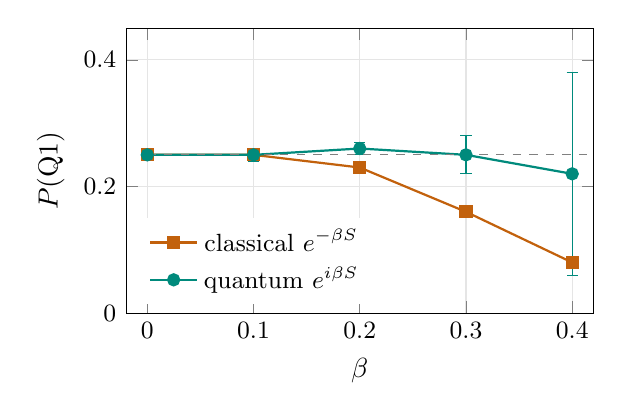
\begin{tikzpicture}
\begin{axis}[width=0.62\textwidth,height=5.2cm,xlabel={$\beta$},ylabel={$P(\mathrm{Q1})$},xtick={0,0.1,0.2,0.3,0.4},
  legend pos=south west,legend style={font=\small,draw=none},grid=major,grid style={gray!20},tick label style={font=\small},
  ymin=0,ymax=0.45,xmin=-0.02,xmax=0.42]
\addplot[thick,bandB,mark=square*] coordinates {(0,0.25)(0.1,0.25)(0.2,0.23)(0.3,0.16)(0.4,0.08)};
\addlegendentry{classical $e^{-\beta S}$}
\addplot[thick,bandA,mark=*,error bars/.cd,y dir=both,y explicit] coordinates {(0,0.25)+-(0,0.00)(0.1,0.25)+-(0,0.01)(0.2,0.26)+-(0,0.01)(0.3,0.25)+-(0,0.03)(0.4,0.22)+-(0,0.16)};
\addlegendentry{quantum $e^{i\beta S}$}
\addplot[dashed,gray] coordinates {(0,0.25)(0.42,0.25)};
\end{axis}
\end{tikzpicture}
\end{center}
Classically, raising $\beta$ drains the most manifold-like quartile (just below the $N=100$ transition). With quantum weights there is no drift within errors up to $\beta=0.3$; at $0.4$ the phases cancel too much to say anything. This agrees with the exact sums. The caveats are real. All sampled universes are genuine sprinklings, so the quartiles compare fluctuations rather than sheets against crystals. Classical reweighting misses rare low-action universes. The quantum errors are $\pm0.03$--$0.06$ at $\beta=0.3$.

\section{Discussion}
\paragraph{Where this sits.} The kinematics is causal set theory: links, infinite valency, Number $=$ Volume, the longest chain as proper time, growth, the Benincasa--Dowker action, the phase transition and the overlap distances are theirs. Our additions are (i) the finite size of the universe as the regulator of the non-locality, with the cosmological frame accepted as a frame of the state; (ii) the rectangle identity~\eqref{eq:rect}; (iii) curvature from the depth drift~\eqref{eq:drift}; (iv) a calibrated, intrinsic manifold detector; and (v) quantum record probabilities by sampling at $N=100$, with the $|A_r|$ bound. Items (ii)--(iv) were not found in brief searches; (v) is a method, and its result is preliminary. On the dynamics side, a cosmological clock (C5) would license writing the sum over histories as a transfer matrix between cosmic-time layers, with operators that create events (C7). That puts us next to causal dynamical triangulations and Hořava--Lifshitz gravity, whose preferred foliation is fundamental rather than emergent; we must show that the difference is real.

\paragraph{Limitations.}
\begin{enumerate}[leftmargin=*,itemsep=1pt]
\item \emph{Everything is $1+1$.} The rectangle identity is $1+1$ only, and $1+1$ GR has no Newtonian limit, so C6 needs $3+1$.
\item \emph{$3+1$ is not tamed}: $10^{124}$ neighbours per event.
\item \emph{No matter.} Nothing gravitates.
\item \emph{Small universes.} The detector needs $N\gtrsim100$--$200$. Exact quantum sums stop at $N\approx12$, and sampled ones are limited by the average phase.
\item \emph{The quantum result is fluctuation-level.} The record (stress quartile) and $\epsilon$ are chosen, not derived.
\item \emph{No prediction yet.} The cutoff is far beyond any test.
\end{enumerate}

\paragraph{Next steps.}
\begin{itemize}[leftmargin=*,itemsep=1pt]
\item Quantum sampling at $N=200$ with $10^6$ samples on the cluster (2--3 core-hours); records that separate sheets from crystals, not just fluctuations.
\item Settle the $N=400$ crystallisation (longer chains of $e^{-\beta S}$ samples).
\item The general Boguñá--Krioukov estimator and the detector in $2+1$ and $3+1$.
\item A relational definition of $L$ and $\eta_{\max}$ in a growing universe; the layer-by-layer operator formulation.
\end{itemize}

\appendix
\section{Paths explored and dropped}\label{app:dropped}
\begin{itemize}[leftmargin=*,itemsep=1pt]
\item \textbf{A regular crystal of events.} Polygonal light cones and a lattice rest frame~\cite{Burago,Weyl}.
\item \textbf{Quantum blur of positions.} Blur in \emph{what}? It presupposes a background, and an equal superposition over rapidity cannot be normalised.
\item \textbf{A quantum chain as the source of blur.} Background-dependent. The atomic-linewidth analogy was overstated: coupling \emph{reduces} the blur.
\item \textbf{Expansion as a source and gravity as a sink of points} (river model~\cite{HamiltonLisle08}). It needs an aether.
\item \textbf{A link to Bell non-locality.} Links are timelike; Bell correlations are spacelike.
\item \textbf{$(L/\lP)^2\sim10^{122}$ and the cosmological constant.} Numerology: every combination of $L$ and $\lP$ is a power of $10^{61}$.
\item \textbf{The manifold detector on exact quantum sums.} At $N\le12$ the detector cannot tell a flat universe from a crystal; replaced by sampling.
\end{itemize}

\begin{thebibliography}{99}\small
\bibitem{JacobsonMattingly01} T.~Jacobson, D.~Mattingly, ``Gravity with a dynamical preferred frame'', Phys.\ Rev.\ D 64, 024028 (2001), gr-qc/0007031.
\bibitem{BLMS87} L.~Bombelli, J.~Lee, D.~Meyer, R.~D.~Sorkin, ``Space-time as a causal set'', Phys.\ Rev.\ Lett.\ 59, 521 (1987).
\bibitem{Surya19} S.~Surya, ``The causal set approach to quantum gravity'', Living Rev.\ Rel.\ (2019), arXiv:1903.11544.
\bibitem{BHS06} L.~Bombelli, J.~Henson, R.~D.~Sorkin, ``Discreteness without symmetry breaking: a theorem'', gr-qc/0605006.
\bibitem{Sorkin07} R.~D.~Sorkin, ``Does locality fail at intermediate length-scales?'', gr-qc/0703099.
\bibitem{CG99} S.~Coleman, S.~L.~Glashow, ``High-energy tests of Lorentz invariance'', Phys.\ Rev.\ D 59, 116008 (1999), hep-ph/9812418.
\bibitem{BrightwellGregory91} G.~Brightwell, R.~Gregory, ``Structure of random discrete spacetime'', Phys.\ Rev.\ Lett.\ 66, 260 (1991).
\bibitem{BDJ99} J.~Baik, P.~Deift, K.~Johansson, ``On the distribution of the length of the longest increasing subsequence of random permutations'', J.\ Amer.\ Math.\ Soc.\ 12, 1119 (1999).
\bibitem{BK24} M.~Boguñá, D.~Krioukov, ``Measuring spatial distances in causal sets via causal overlaps'', Phys.\ Rev.\ D 110, 024008 (2024), arXiv:2401.17376.
\bibitem{BD10} D.~M.~T.~Benincasa, F.~Dowker, ``The scalar curvature of a causal set'', Phys.\ Rev.\ Lett.\ 104, 181301 (2010).
\bibitem{DowkerGlaser13} F.~Dowker, L.~Glaser, ``Causal set d'Alembertians for various dimensions'', arXiv:1305.2588.
\bibitem{GibbonsSolodukhin07} G.~W.~Gibbons, S.~N.~Solodukhin, ``The geometry of small causal diamonds'', Phys.\ Lett.\ B 649, 317 (2007), hep-th/0703098.
\bibitem{RSS13} M.~Roy, D.~Sinha, S.~Surya, ``The discrete geometry of a small causal diamond'', Phys.\ Rev.\ D 87, 044046 (2013), arXiv:1212.0631.
\bibitem{Johnston25} S.~Johnston, ``Simpler embeddings of causal sets into Minkowski spacetime'', arXiv:2502.09701.
\bibitem{RideoutSorkin00} D.~P.~Rideout, R.~D.~Sorkin, ``A classical sequential growth dynamics for causal sets'', Phys.\ Rev.\ D 61, 024002 (2000).
\bibitem{MORS01} X.~Mart\'in, D.~O'Connor, D.~P.~Rideout, R.~D.~Sorkin, ``On the renormalization transformations induced by cycles of expansion and contraction in causal set cosmology'', Phys.\ Rev.\ D 63, 084026 (2001).
\bibitem{AhmedRideout10} M.~Ahmed, D.~Rideout, ``Indications of de Sitter spacetime from classical sequential growth dynamics of causal sets'', Phys.\ Rev.\ D 81, 083528 (2010).
\bibitem{Surya12} S.~Surya, ``Evidence for a phase transition in 2D causal set quantum gravity'', arXiv:1110.6244.
\bibitem{BHS08} G.~Brightwell, J.~Henson, S.~Surya, ``A 2D model of causal set quantum gravity: the emergence of the continuum'', arXiv:0706.0375.
\bibitem{GOS18} L.~Glaser, D.~O'Connor, S.~Surya, ``Finite size scaling in 2d causal set quantum gravity'', Class.\ Quant.\ Grav.\ (2018), arXiv:1706.06432.
\bibitem{Burago} D.~Burago, ``Periodic metrics''; statement in arXiv:1104.4460.
\bibitem{Weyl} H.~Weyl, \emph{Philosophy of Mathematics and Natural Science} (1949).
\bibitem{HamiltonLisle08} A.~J.~S.~Hamilton, J.~P.~Lisle, ``The river model of black holes'', Am.\ J.\ Phys.\ 76, 519 (2008).
\end{thebibliography}
\end{document}
